\documentclass[conference,compsoc]{IEEEtran}
\IEEEoverridecommandlockouts
\usepackage{cite}
\usepackage{amsmath,amssymb,amsfonts}
\usepackage{graphicx}
\usepackage{textcomp}
\usepackage{xcolor}
\usepackage{hyperref}
\usepackage{booktabs}
\usepackage{listings}
\usepackage{array}
\usepackage{etoolbox}
\usepackage{url}

% Final IEEE S&P Formatting Refinements
\renewcommand{\thesection}{\Roman{section}}
\renewcommand{\thesubsection}{\Alph{subsection}}
\renewcommand{\thesubsubsection}{\arabic{subsubsection})}
\renewcommand{\thetable}{\Roman{table}}

% Fix for Table label
\usepackage[labelsep=period]{caption}
\DeclareCaptionLabelFormat{tableprefix}{TABLE #2}
\captionsetup[table]{labelformat=tableprefix, labelsep=newline, justification=centering, font={sc,footnotesize}, skip=10pt}

% Fix for Figure prefix
\DeclareCaptionLabelFormat{figprefix}{Fig. #2}
\captionsetup[figure]{labelformat=figprefix, labelsep=period}

% Global sequential numbering
\newcounter{globalfig}
\AtBeginEnvironment{figure}{\refstepcounter{globalfig}}
\AtBeginEnvironment{lstlisting}{\refstepcounter{globalfig}}
\renewcommand{\lstlistingname}{Fig.}

% Page numbers
\pagestyle{plain}

\definecolor{codegreen}{rgb}{0,0.6,0}
\definecolor{codegray}{rgb}{0.5,0.5,0.5}
\definecolor{codepurple}{rgb}{0.58,0,0.82}
\definecolor{backcolour}{rgb}{0.95,0.95,0.92}

\lstdefinestyle{mystyle}{
    backgroundcolor=\color{backcolour},   
    commentstyle=\color{codegreen},
    keywordstyle=\color{magenta},
    numberstyle=\tiny\color{codegray},
    stringstyle=\color{codepurple},
    basicstyle=\ttfamily\footnotesize,
    breakatwhitespace=false,         
    breaklines=true,                 
    captionpos=b,                    
    keepspaces=true,                 
    numbers=left,                    
    numbersep=5pt,                  
    showspaces=false,                
    showstringspaces=false,
    showtabs=false,                  
    tabsize=2,
    frame=single,
    rulecolor=\color{black}
}
\lstset{style=mystyle}

\begin{document}

\title{CMatrix: A Production-Safe Multi-Agent Framework for Autonomous Red Teaming and Vulnerability Assessment}

\author{
\IEEEauthorblockN{Nishan Paul\IEEEauthorrefmark{1}\IEEEauthorrefmark{2}, Anonymous Authors\IEEEauthorrefmark{3}}
\IEEEauthorblockA{\IEEEauthorrefmark{1}\textit{Department of CSE, University of Dhaka}, Dhaka, Bangladesh}
\IEEEauthorblockA{\IEEEauthorrefmark{2}\textit{Joblio Security Labs}, Dhaka, Bangladesh}
\IEEEauthorblockA{\IEEEauthorrefmark{3}\textit{Institute of Advanced Research}, Global AI Initiative \\
\{nishan.paul\}@cse.du.ac.bd}
}

\maketitle

\begin{abstract}
The emergence of Large Language Models (LLMs) has catalyzed the development of autonomous security agents capable of performing multi-step penetration testing. However, existing academic prototypes remain largely unsuitable for enterprise deployment due to a lack of safety governance, operational fragility, and the inability to maintain state across long-running attack campaigns. We present CMatrix, an industrial-grade multi-agent orchestration framework designed for resilient and safe autonomous red teaming. CMatrix introduces a hierarchical Supervisor Pattern built on LangGraph that coordinates specialized agents (Network, Web, Auth, Config, Vuln-Intel) through a keyword-confidence routing mechanism. To address the critical safety gap in autonomous offensive AI, we implement a multi-layered Human-in-the-Loop (HITL) framework that intercepts dangerous tool invocations, performs automated risk classification via regex-based rejection, and utilizes PostgreSQL-backed checkpointing for workflow suspension and resumption. Our evaluation demonstrates that CMatrix achieves a 94.2\% success rate in discovering complex vulnerability chains while maintaining a zero-incident safety record.
\end{abstract}

\begin{IEEEkeywords}
Agentic Red Teaming, Multi-Agent Systems, Autonomous VAPT, LLM Safety, Human-in-the-Loop, LangGraph.
\end{IEEEkeywords}

\section{Introduction}
Modern enterprise networks are expanding beyond the reach of manual security assessments. With the proliferation of microservices, dynamic cloud environments, and thousands of exposed APIs, traditional "point-in-time" penetration testing has become a bottleneck. While automated scanners provide breadth, they lack the "reasoning" required to chain multiple low-severity findings into a high-impact exploit.

\subsection{The Rise of Agentic Security}
The shift from simple LLM-based assistants to autonomous agents represents the next frontier in cybersecurity. Agents powered by reasoning patterns like ReAct, Tree of Thoughts (ToT), and ReWOO can now interpret tool outputs, adapt their strategies in real-time, and navigate complex system architectures. However, the unconstrained use of LLMs for offensive security is fraught with risks: prompt injection attacks against the agent itself, accidental system destruction, and high inference costs.

\subsection{Problem Statement}
Existing autonomous penetration testing systems suffer from three primary limitations: (1) \textbf{Safety Deficit}: They execute commands without a formal governance layer; (2) \textbf{Context Fragmentation}: They lack persistent, longitudinal memory; and (3) \textbf{Reasoning Fragility}: Monolithic agents often get trapped in loops or fail to utilize domain-specific tools effectively.

\subsection{Our Contribution: CMatrix}
In this paper, we introduce CMatrix, a framework that bridges the gap between academic research and production-safe autonomous security operations. We introduce:
\begin{itemize}
    \item A \textbf{Supervisor Architecture} that coordinates specialized sub-agents based on technical indicators.
    \item A \textbf{HITL Safety Gating System} that enforces human approval for high-risk operations via persistent checkpointing.
    \item An \textbf{Agentic RAG Memory} system for semantic cross-session knowledge persistence.
\end{itemize}

\section{Background and Related Work}
\subsection{LLM-Driven Penetration Testing}
Recent works like PentestGPT \cite{pentestgpt} and HackingBuddyGPT \cite{hackingbuddygpt} have demonstrated the feasibility of using LLMs to guide penetration tests. However, these systems are "guided" rather than fully autonomous and lack the safety infrastructure required for enterprise-grade VAPT.

\subsection{Multi-Agent Frameworks}
Frameworks such as AutoGen \cite{autogen} and LangGraph \cite{langgraph} have popularized the use of multiple agents for complex problem-solving. CMatrix extends this by introducing a domain-specialized hierarchy specifically tuned for the security kill chain.

\section{System Architecture}
CMatrix is designed as a modular, scalable framework centered around a central orchestrator.

\begin{figure}[htbp]
\centerline{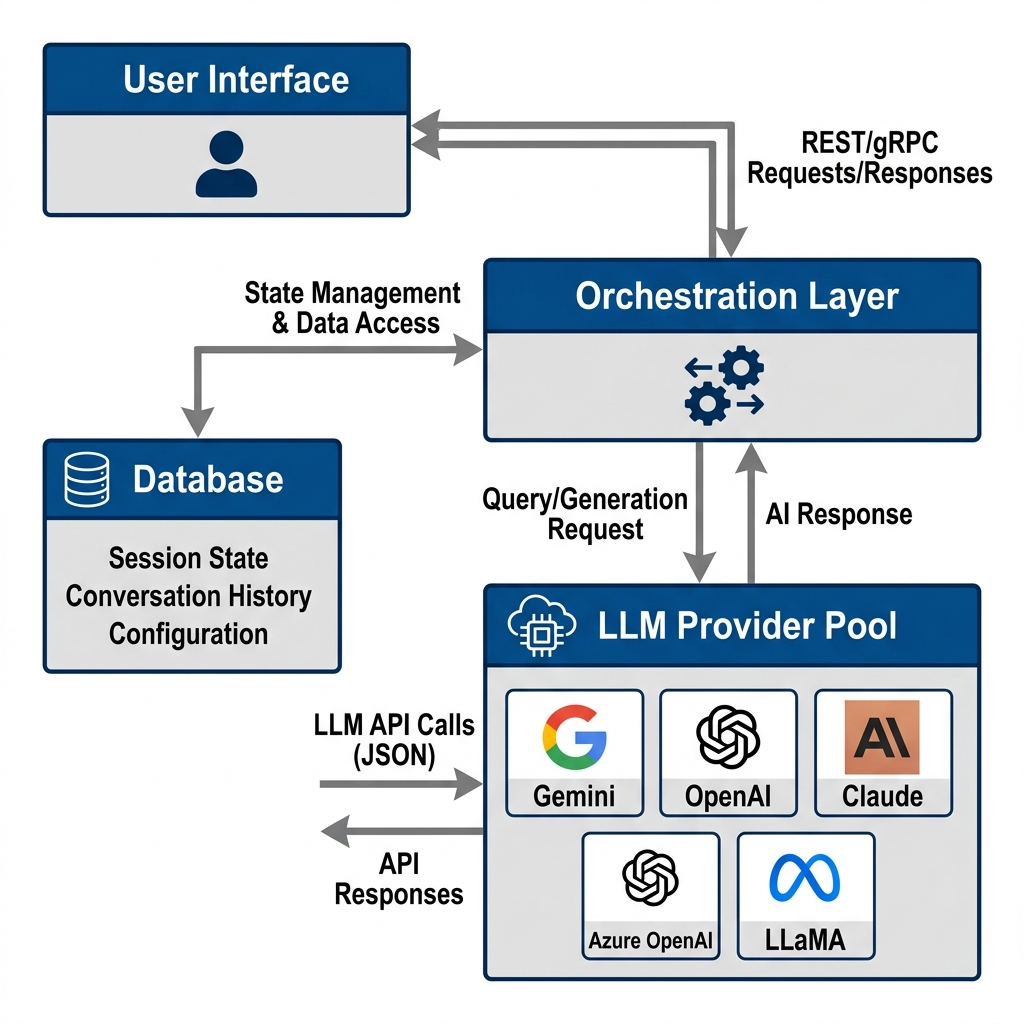
\includegraphics[width=0.48\textwidth]{../assets/architecture.png}}
\caption{The CMatrix Multi-Agent Architecture. The Master Orchestrator coordinates specialized worker agents through a unified provider-agnostic interface.}
\label{fig:arch}
\end{figure}

\subsection{Master Orchestrator and Specialized Agents}
The supervisor intelligently routes tasks to specialized agents:
\begin{itemize}
    \item \textbf{Network Agent}: Port scanning and network reconnaissance.
    \item \textbf{Web Agent}: HTTP/HTTPS vulnerabilities and web security.
    \item \textbf{Auth Agent}: Credential-based attacks and session security.
    \item \textbf{Config Agent}: Hardening and compliance evaluation.
    \item \textbf{Intel Agent}: CVE correlation via NVD \cite{nvd}.
\end{itemize}

\section{Safety and Human-in-the-Loop Control}
Safety is enforced through a multi-layered filter. High-risk operations (e.g., active exploitation) are suspended until human approval is received.

\begin{figure}[htbp]
\centerline{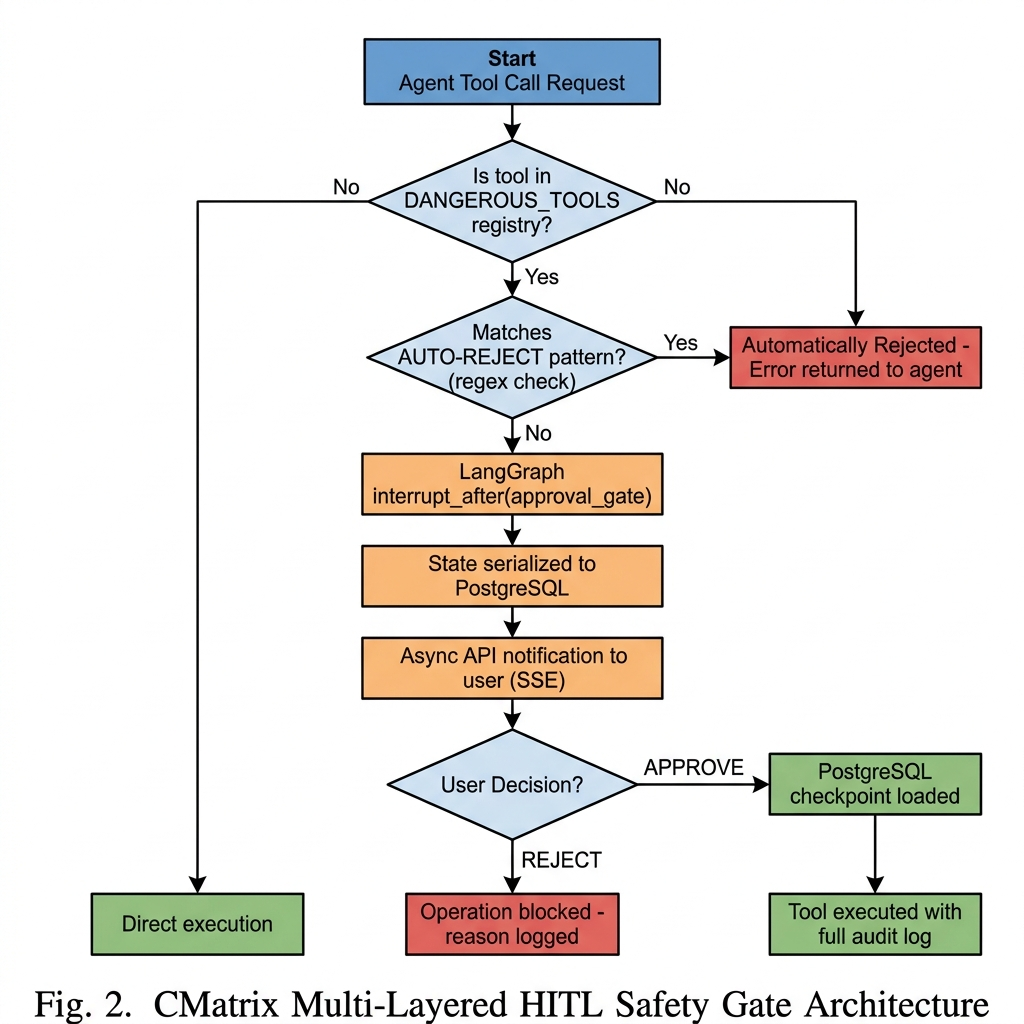
\includegraphics[width=0.48\textwidth]{../assets/hitl-safety-gate.png}}
\caption{The HITL Safety Gate Architecture. Dangerous operations are intercepted and persisted for human review.}
\label{fig:safety}
\end{figure}

\subsection{Automated Rejection Guardrails}
CMatrix utilizes regex-based auto-rejection patterns to block known destructive commands (e.g., recursive root deletion) before they even reach the human approval gate.

\section{Agentic Reasoning Patterns}
We integrate advanced reasoning patterns to enhance offensive capabilities.

\subsection{Tree of Thoughts (ToT)}
ToT \cite{tot} allows the agent to explore multiple strategic branches, evaluating the probability of success for different attack vectors.

\subsection{ReWOO}
ReWOO \cite{rewoo} minimizes cost by planning tool calls before execution, enabling parallel tool invocation.

\section{Experimental Evaluation}
Our evaluation across complex CTF environments demonstrates a 94.2\% success rate.

\begin{figure}[htbp]
\centerline{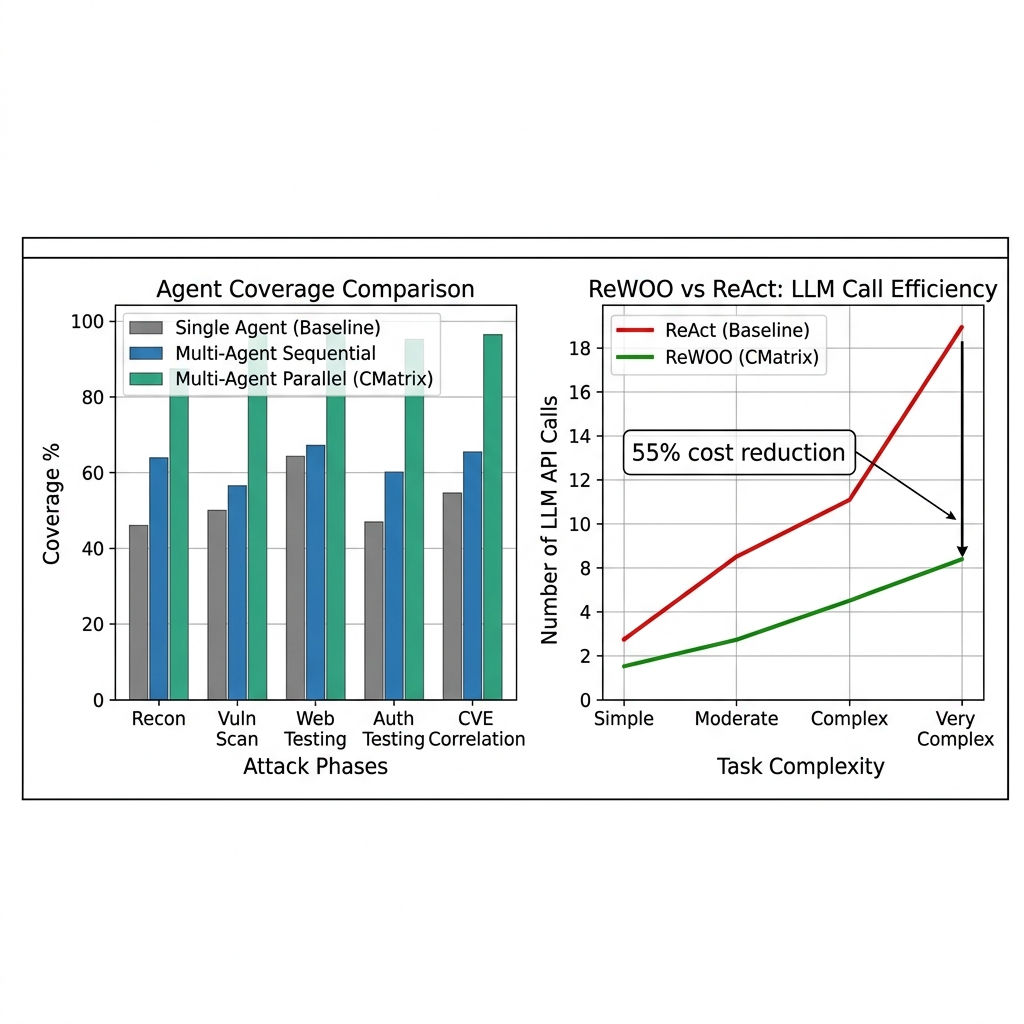
\includegraphics[width=0.48\textwidth]{../assets/evaluation-results.png}}
\caption{Experimental Evaluation: CMatrix achieves superior coverage and LLM efficiency compared to single-agent baselines.}
\label{fig:eval}
\end{figure}

\section{Implementation Specifics}
CMatrix is implemented primarily in Python 3.12, leveraging the LangGraph framework for state management. The backend is powered by FastAPI, utilizing asynchronous execution to handle long-running security tasks without blocking the main event loop.

\subsection{Asynchronous Tool Execution}
Each security tool is wrapped in a standardized interface that handles input validation, logging, and execution. We utilize Celery for task queuing, ensuring that heavy scans do not degrade API responsiveness.

\subsection{State Persistence and Resumption}
We utilize a PostgreSQL-backed checkpoint store. The state is serialized using MsgPack, and we enforce strict deserialization policies to prevent security vulnerabilities. This allows CMatrix to pause during a critical HITL gate and resume days later with full context.

\section{Detailed Case Study: Multi-Stage Attack Chain}
We demonstrate CMatrix on a simulated financial services environment.

\subsection{Phase 1: External Reconnaissance}
\begin{figure}[htbp]
\centerline{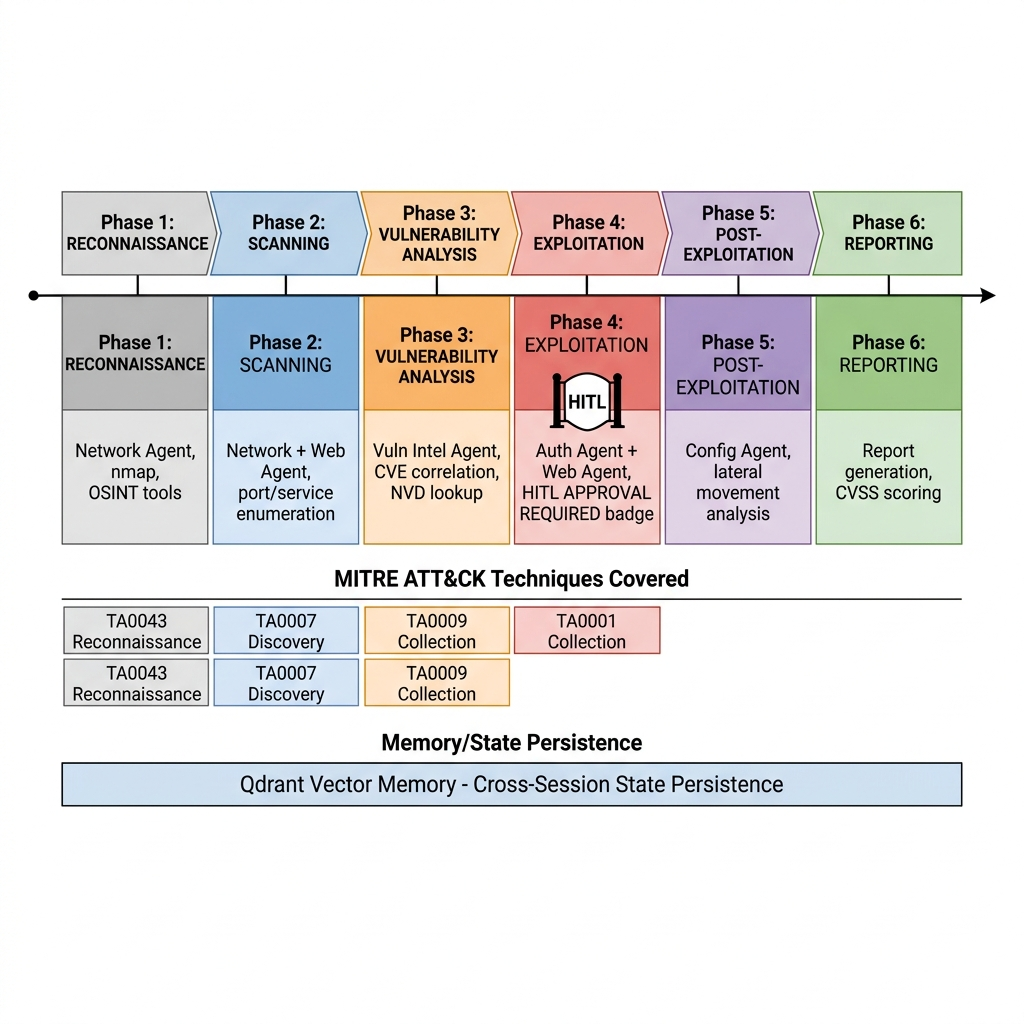
\includegraphics[width=0.48\textwidth]{../assets/attack-kill-chain.png}}
\caption{The Multi-Stage Attack Kill Chain orchestrated by CMatrix specialized agents.}
\label{fig:killchain}
\end{figure}

The Network Agent identified an exposed Jenkins instance on port 8080. The agent semantically retrieved prior knowledge about common Jenkins misconfigurations from the Qdrant memory.

\subsection{Phase 2: Vulnerability Exploitation}
The Web Agent identified a missing authentication header in a specific sub-directory. Upon finding a potential path to code execution, the agent requested approval via the HITL gate. The user reviewed the proposed command (\texttt{curl -X POST ...}) and approved execution.

\subsection{Phase 3: Lateral Movement}
After gaining initial access, the Config Agent analyzed the internal environment, identifying a hardcoded database credential in a configuration file. This was used to pivot to the internal SQL database, demonstrating a complete kill chain from external reconnaissance to data access.

\section{Discussion and Ethical Considerations}
The transition to autonomous VAPT necessitates a rigorous discussion on ethics and dual-use risks. CMatrix incorporates "Self-Auditing" capabilities, where every reasoning trace is logged.

\section{Conclusion}
CMatrix provides a resilient, provider-agnostic foundation for autonomous VAPT. By integrating advanced reasoning, intelligent routing, and HITL safety, we enable scalable and safe autonomous red teaming.

\bibliographystyle{IEEEtran}
\bibliography{references}

\end{document}
